\documentclass[review]{elsarticle}

\usepackage{lineno,hyperref}
\usepackage{listings}
\usepackage{amsthm, amsmath,amssymb,amsbsy,amsfonts,amstext,rotating}
\usepackage{alltt,multicol,pifont}
\usepackage{booktabs,multirow,subfigure,epsfig}
\usepackage{xspace}
\newcommand{\eplopmark}{\ding{73}}
\usepackage{url}
\usepackage{tipa}
\usepackage{array,tabularx}
\usepackage{color}
\definecolor{applegreen}{rgb}{0.55, 0.71, 0.0}
\definecolor{bananayellow}{rgb}{1.0, 0.88, 0.21}
\definecolor{blue}{rgb}{0.0, 0.53, 0.74}

% *** ALIGNMENT PACKAGES ***
%
\usepackage{array,tabularx}
\modulolinenumbers[5]

\renewcommand{\arraystretch}{0.7}

\journal{Journal of Biomedical Informatics}

%%%%%%%%%%%%%%%%%%%%%%%
%% Elsevier bibliography styles
%%%%%%%%%%%%%%%%%%%%%%%
%% To change the style, put a % in front of the second line of the current style and
%% remove the % from the second line of the style you would like to use.
%%%%%%%%%%%%%%%%%%%%%%%

%% Numbered
%\bibliographystyle{model1-num-names}

%% Numbered without titles
%\bibliographystyle{model1a-num-names}

%% Harvard
%\bibliographystyle{model2-names.bst}\biboptions{authoryear}

%% Vancouver numbered
%\usepackage{numcompress}\bibliographystyle{model3-num-names}

%% Vancouver name/year
%\usepackage{numcompress}\bibliographystyle{model4-names}\biboptions{authoryear}

%% APA style
%\bibliographystyle{model5-names}\biboptions{authoryear}

%% AMA style
%\usepackage{numcompress}\bibliographystyle{model6-num-names}

%% `Elsevier LaTeX' style
\bibliographystyle{elsarticle-num}
%%%%%%%%%%%%%%%%%%%%%%%

\begin{document}

\begin{frontmatter}

\title{Test event generation for a fall-detection IoT system}

%% Group authors per affiliation:

\author{Lorena Guti\'errez-Madro\~nal\fnref{label1}}
%% \author{Name\corref{cor1}\fnref{label2}}
\ead{lorena.gutierrez@uca.es (corresponding author)}
\author{Luigi La Blunda\fnref{label2}}
\ead{l.lablunda@fb2.fra-uas.de}
\author{Matthias F. Wagner\fnref{label2}}
\ead{mfwagner@fb2.fra-uas.de}
\author{I. Medina-Bulo\fnref{label1}}
\ead{inmaculada.medina@uca.es}
\address[label1]{UCASE Software Engineering Research group, University of 2. C\'adiz, Av. Universidad de 2. C\'adiz, 10, 11519 Puerto Real, Spain.}
\address[label2]{WSN and IOT Research Group Frankfurt University of Applied Sciences.}


\begin{abstract}
The Internet of Things (IoT) is a popular paradigm which has been applied to different areas 
such as smart cities, medicine or business processes. One of the main drawbacks of an IoT system is the 
amount of information they have to manage and to monitor. This information arrives as events that need 
to be processed in real time in order to make correct decisions. The Event Processing Languages were 
designed to handle this information by defining event patterns which describe relevant situations to be 
detected and filter the information. 
In the majority of the relevant situations to detect, the events have a specific behaviour which must be analysed
not only to define the event patterns, but also to simulate them to test the IoT system. Moreover, in several 
situations it is quite difficult to obtain test events with specific values: adverse environment conditions, 
rise or fall in blood pressure, heart attack, falls, among others. 
In this paper we introduce a complete study of falls as relevant situations; we show an analysis of the fall-involved
events of two type of falls base on an IoT prototype, the event patterns to detect the falls and their test using 
the IoT-TEG (IoT - Test Event Generator) tool. The fall analysis has highlighted the necessity to improve IoT-TEG 
with a new functionality which allows defining the desired conduct by defining behaviour rules.
\end{abstract}

\begin{keyword}
event generator\sep testing\sep Internet of Things\sep Complex Event Processing\sep fall detection\sep behaviour rules
\end{keyword}

\end{frontmatter}

\section{Introduction}

Due to the progress of health care, the longevity of people increases and this leads to an ageing society. %Elderly people are exposed 
%to a higher risk of falling because of the growing age and multiple diseases, which cause serious injuries that require long convalescence 
%and restriction of mobility. 
According to the survey of the \textit{Robert Koch Institute}~\cite{Varnaccia2013}, 53.7\% of accidents in the age 
group over 60 are caused by falls. Statistically, about one-third of the elderly people suffer severe lesions and the half of them suffer 
fall-events repeatedly~\cite{Schott2008}. Falls are not caused by a single cause, 90\% of them occurred from multiple factors. These 
factors refer to old-age or illness (intrinsic factors) or external factors e.g. hazards which occur at home, in traffic or during activities 
of daily life (extrinsic factors)~\cite{Schott2008}. The founder of \textit{Vigilio Telemedical} reported that yearly more than 20 million 
elderly over the age of 65 in Europe experience fall-situations, that lead to traumatic based cases of death~\cite{Vigilio,APAOTS2013}. 
Additionally, people affected by Dementia and Parkinson have a higher risk to fall. In accordance with~\cite{Monks} research proved that 
Dementia-patients have a 20 times higher risk and Parkinson-patients a 10 times higher risk of falling than healthy people of the same age. 
To counteract these life-threatening situations a fast and fully automated assistance is needed, because an unconscious person may not be 
able to call the emergency services. An approach could be continuous monitoring of medical and/or physical signals via a wearable sensor 
network (see Figure~\ref{fig:escalationscheme}). A prototype in form of a belt was developed, which is worn on the hip by the patient and consists 
of a five sensor nodes Body Area Network (BAN)~\cite{LaBlunda.2016,LaBlunda.2016b}. 

\begin{figure}[!ht]
  \centering
  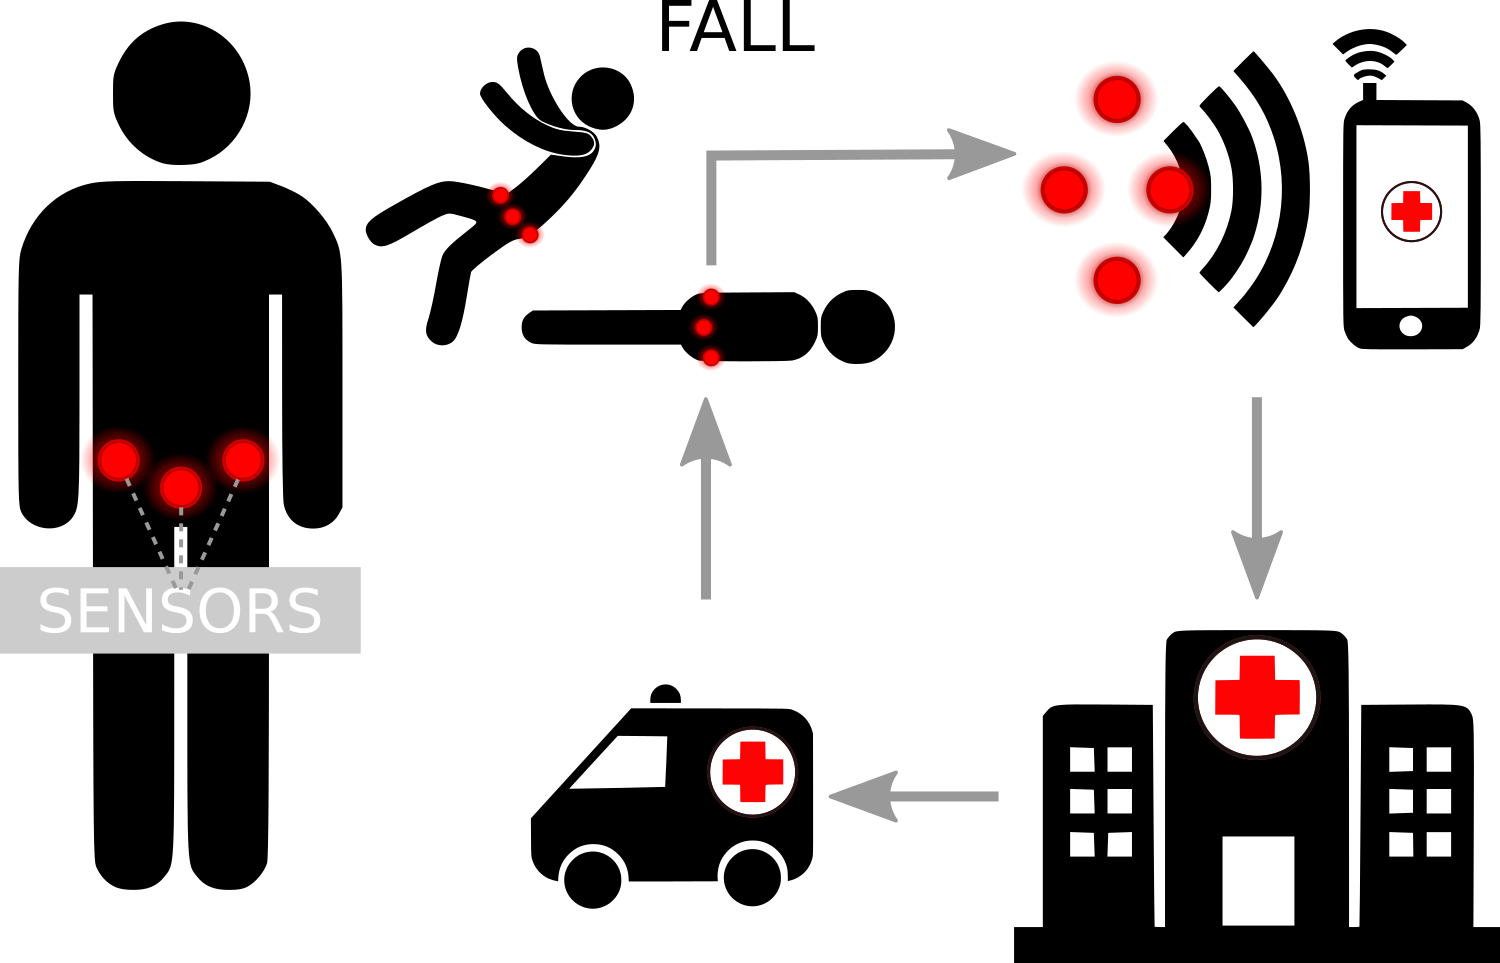
\includegraphics[scale=0.15]{img/Figure1}
  \caption[Escalation scheme]{Scheme fall simulation where a person has a wareable sensor network in form of a belt.~\cite{LaBlunda.2016,LaBlunda.2016b}}
  \label{fig:escalationscheme}
\end{figure}

The Event processing languages (EPLs) have been designed to address the main problems of 
IoT systems. In particular, EPLs are used to define critical situations in order to filter the 
information and to make correct decisions according to the obtained data. These critical 
situations are defined using event patterns and event rules. Among the existing EPLs, the 
EPL of EsperTech~\cite{Esper:2016} is used the most often. In our study, the critical situations are the falls,
so the obtained data from the mentioned prototype are used to define an EPL of EsperTech 
pattern to detect falls.

The first step of this prototype is to identify a fall from a fast movement, a sitting move or laying 
down move, but the final goal of the system is to predict the falls and act to prevent 
them. Given that to test this system is crucial, test events which simulate falls are necessary. In 
the literature different type of falls can be found, and it is necessary to identify all of them in 
order to tell them apart from a no-fall: in this study two types of falls will be analysed. 

IoT-TEG~\cite{TesisGutierrez2017,Gutierrez2017} is a tool which automatically generates test events 
of many types. Thanks to the obtained data from the sensors we have checked that the measured 
parameter during a fall, the acceleration, has a specific behaviour. As a consequence, the test events 
must be generated according to its behaviour. This problem is solved with the new functionality that 
IoT-TEG includes which is introduced in this paper. %Moreover, the ongoing fall detection prototype will 
%be analysed and its improvements will be described; the new functionality of IoT-TEG can be adapted 
%according to the improvements of the fall detection prototype. 

In this study of falls as relevant situations, our main contributions are:

\begin{itemize}
\item \textbf{A study of the fall detection prototype evolution}: the system which is been used is
 continuously being improved. We describe the evolution of its architecture, how the data is analysed and 
 the detected problems.
 \item \textbf{An analysis of the major parameter in a fall}: while a person is falling, the acceleration 
 is the parameter that can measure the movement of the body. This parameter is analysed in order to know 
 its behaviour during two types of falls.
 \item \textbf{New definitions of two types of falls}: after the analysis of the acceleration during two 
 types of falls a new definition for each one has been done. The obtained data of the fall detection 
 prototype is used to define EPL of EsperTech patterns to detect those type of falls. 
 \item \textbf{A new functionality of the IoT-TEG system} which allows to simulate the behaviour of 
 different event attributes in order to generate test events following a specific pattern. 
\end{itemize}

The rest of this paper is organised as follows. Section~\ref{sec:relatedwork}
describes not only the related work of event generators, but also the existing
solutions for fall-detection. Section~\ref{sec:background} provides the basic
knowledge of falls, Event Processing Languages and IoT-TEG tool. The architecture
of the fall detection system, the fall analysis and the IoT-TEG new functionality are 
introduced in Section~\ref{sec:basicprototype}. Section~\ref{sec:improvedprototype}
describes the improvements on the prototype, a new fall type analysis,
a comparison of the obtained results and some detected problems. Finally, in Section~\ref{sec:conclusions}, 
we conclude our paper and make recommendations for future work.

\section{Related work}
\label{sec:relatedwork}

An overview about event generators reveals that the first event generators~\cite{dobbs2004houches,mangano2005tools}
were focused on extremely specific topics such as environmental conditions for the simulation of high energy 
physics events at particle colliders. Nowadays, we can find papers that address the same issues~\cite{Grzegorczyk}, but 
the technology surrounds us and the people and business need to control and monitor the things around them. 
The received information allows them to make decisions and to act according to it. This is the reason 
of the creation of the IoT platforms, which are the key for the development of scalable IoT applications and 
services that connect objects, systems and people to each other. However, not every IoT platform is a real IoT 
platform~\cite{iot-analytics:2015}; for instance, some event generators that are integrated in an enterprise 
software packages, which are increasingly allowing the integration of IoT devices, are often not advanced enough
to be classified as a full IoT platform. Examples are given in the following lines:

\begin{itemize}
 \item The Timing System~\cite{Finland:2016} provides a complete timing distribution system including timing signal 
 generation. Its event generator is responsible for creating timing events which are sent out as serialised event frames.
 \item The company Starcom~\cite{Starcom:2016} has developed an event generator to solve the problem of managing a huge 
 number of events. They state that their generator is capable of controlling the end event action, so the exact managers 
 requirements can be filtered. The tool is included in a kit distributed with their system.
 \item The WebLogic Integration Solutions~\cite{WebLogic:2016} allow the managing and monitoring of entities and 
 resources required for WebLogic Integration applications. This system contains an event generator module which allows the 
 creation and deployment of the event generators included as part of WebLogic Integration. The mentioned events 
 generators allow to define event types but they are not capable to simulate a specific behaviour with a set of 
 generated events. The relevant situations in IoT systems are a sequence of activities with a determined behaviour; 
 that is why IoT-TEG~\cite{TesisGutierrez2017,Gutierrez2017} includes this option.
\end{itemize}

% Talking about fall-detection, there are several solutions that propose wearable sensors.
% A commercial solution which is 
% available on the market is the VigiFall system~\cite{Vigilio,EuropeanCommission2013}, supported by the European Commission. This system 
% includes a wearable self-adhesive accelerometer, several motion sensors which are fixed in the living area and a calling unit to provide 
% a fully automated emergency call. The self-adhesive patch communicates with the infrared motion detectors and in the case of a fall the 
% wearable patch sends a signal out. Thereby the infrared sensors placed in the room are capable to recognise that there are no movements anymore and 
% contacts the central unit. When the central node receives this flag, the emergency call is executed. The weak point of VigiFall~\cite{Vigilio} is 
% the system structure which depends on the sensor-based room infrastructure. Once the patient leaves this area the system is not capable 
% to provide the functionalities in case of a fall-event. Igual et al.~\cite{Igual2013} examined different fall-detection approaches which they 
% categorised into context-aware systems and wearable systems. Context-aware systems depend on the living area of the patient, where 
% sensors and actuators placed in the environment interact with the wearable node of the person to detect falls. Another solution based 
% on this principle is a video-based method, which facilitates a reliable detection of falls but the patients would be exposed to a 
% loss of privacy and this is not well accepted. Additionally the high purchase price is a barrier for many people and the dependency 
% on the environment makes these system useless. The other system-type analysed by Igual et al.~\cite{Igual2013} comprises wearable systems, which 
% are worn on the body and based on a BAN. This solution is able to detect falls independent from the environment in contrast to 
% context-aware systems. They depict wearable systems which use the sensor fusion principle of accelerometer and gyroscope 
% and built-in solutions that represent the usage of integrated
% smartphone sensors. Collado Villaverde et. al ~\cite{colladoTriaxal}
% use a smartwatch for acquiring accelerometer data and machine learning
% methods to detect a fall event.

%Taking into consideration 

Talking about fall-detection, there are several solutions that propose wearable sensors.
We are going to focus our attention in the approach proposed by Li et al.~\cite{Li2009}; their wearable fall-detection solutions,
which will be explained subsequently, was used for the development of our prototype. They introduce a fall-detection method based on a BAN that consists 
of two wearable sensor nodes. These two nodes comprise an accelerometer and gyroscope and are worn on the chest, node A, and thigh 
node B, (see Figure~\ref{fig:simulation}). The principle of this method differentiates between static postures and dynamic postures: 

\begin{itemize}
 \item Static postures: standing, sitting, laying and bending.
 \item Dynamic postures
 \begin{itemize}
  \item Activities of daily life: walking, walk on stairs, sit, jump, lay down and run.
  \item Fall-like motions: quick sit down upright and quick sit-down reclined.
  \item Flat surface falls: fall forward, fall backward, fall right and fall left.
  \item Inclined falls: fall on stairs.
 \end{itemize}
\end{itemize}

\begin{figure}[!ht]
  \centering
  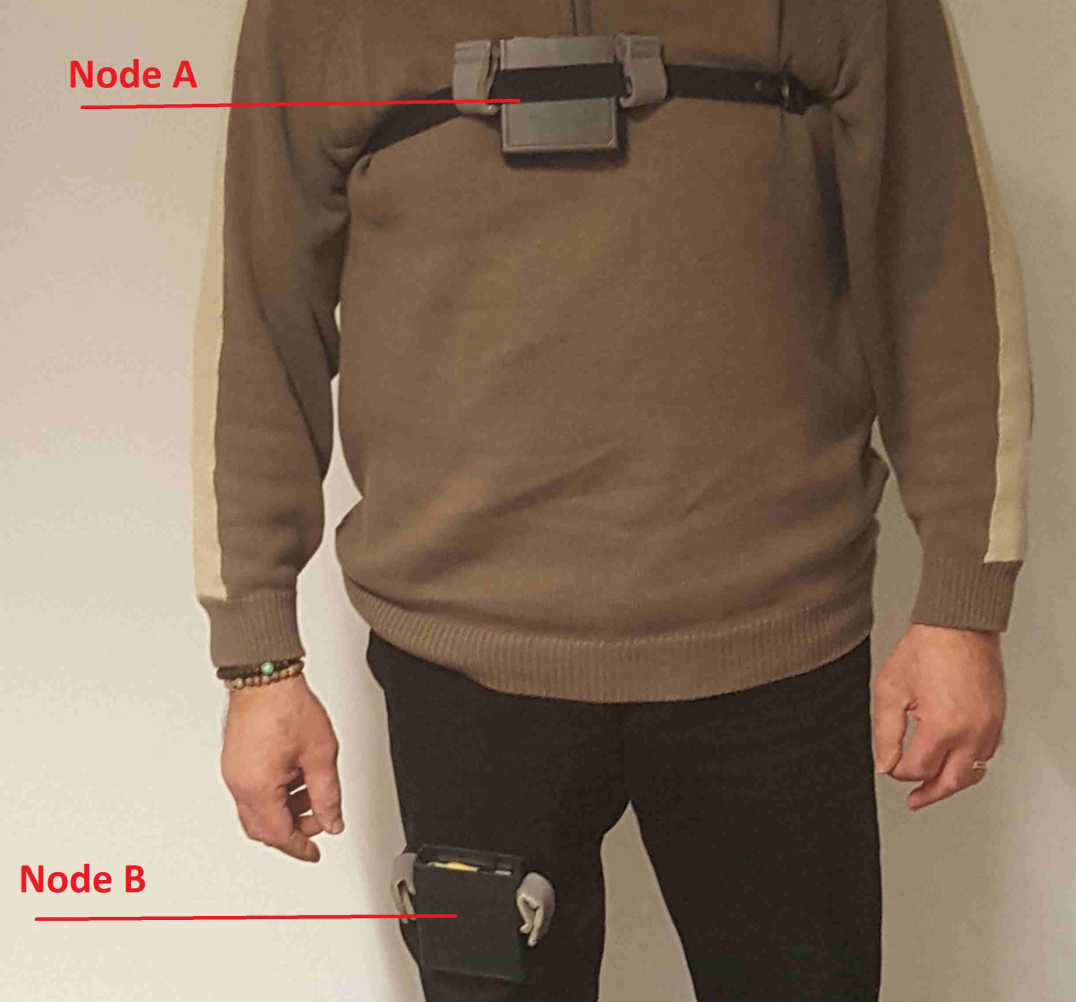
\includegraphics[scale=0.15]{img/BasePrototype.png}
  \caption[System architecture]{System architecture according to Li et al.~\cite{Li2009}}
  \label{fig:simulation}
\end{figure}

To decrease the computational effort of the micro-controller a three-phase algorithm was proposed, which is structured 
as follows:

\begin{enumerate}
 \item Phase activity analysis: check if person is in a static or dynamic position.
 \item Phase position analysis: if existing posture coincides with static posture, check whether the current position corresponds to laying.
 \item Phase state transition analysis: if in laying position, examine whether this transition was intentional or unintentional. The previous 5 
 seconds are used to analyse it. In the case that this position was unintentional, the system classifies it as a fall. 
\end{enumerate}

The weak point of this method is the differentiation between jumping into bed and falling against a wall with seated posture.

\section{Background}
\label{sec:background}

\subsection{Fall analysis}
\label{subsec:analysis}

The approach used to detect falls is based on the basic idea proposed by~\cite{Gjoreski2014,Kozina}. A typical acceleration pattern during 
a fall-event is a decreasing acceleration close to 0g (free fall), followed by an increasing acceleration value (see Figure~\ref{fig:grafica}). In a stationary position, 
the acceleration measured is around 1g (9.81$m/s^{2}$) and during falling around 0g (0$m/s^{2}$). Upon the impact to the ground (fall-event), 
the maximum acceleration (peak-value) is reached for a short time period and it is greater than 1g. This pattern can be used to 
detect fall-events using the integrated accelerometer of the sensor nodes. Important to know is that the acceleration 
magnitude which is illustrated in the Formula~\ref{eq:acel} was used for the fall-detection:

\begin{equation}\label{eq:acel}
 \alpha = \sqrt{\alpha_{x}^{2} + \alpha_{y}^{2} + \alpha_{z}^{2}}
\end{equation}

\begin{figure}[!ht]
  \centering
  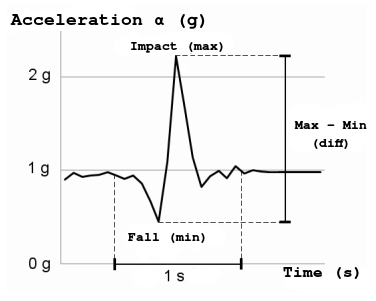
\includegraphics[scale=0.6]{img/FallGraph}
  \caption[Acceleration during impact]{Acceleration during impact~\cite{Kozina}.}
  \label{fig:grafica}
\end{figure}

Taking into consideration the depicted Figure~\ref{fig:grafica}, we can apply the following rule to evaluate the incoming acceleration data:

\begin{equation}\label{eq:caida}
 \alpha_{max} - \alpha_{min} > 1g
\end{equation}

in a 1 second window and $\alpha_{min}$ preceded $\alpha_{max}$; where $\alpha_{max}$ is the maximum acceleration value, 
$\alpha_{min}$ is the minimum acceleration value and $1g\approx9.81m/s^{2}$. Looking at the rule an event is categorised as a fall when the 
difference between $\alpha_{max}$ and $\alpha_{min}$ is greater than 1g and $\alpha_{min}$ is followed by $\alpha_{max}$. 
Important: this should happen within a time window of 1 second due to the fact, that a fall can occur in less than 1 second~\cite{Luder2009}.
To apply this rule we used the Event Processing Language (EPL) of EsperTech~\cite{Esper:2016} to integrate it in an IoT system which detects falls.

\subsection{Fall patterns with EPL of EsperTech}

Etzion and Niblett~\cite{Etz10} defined \textit{event processing agents} as software modules that process events. Such agents are specified using an 
EPL, and there are a number of styles of EPLs in use. The following styles are included: rule-oriented, imperatives and stream-oriented.

% \begin{itemize}
%  \item Rule-oriented languages
%  \begin{itemize}
%  \item Production rules: Production rules are rules of the type \textit{if condition then action}: when the condition is satisfied, the action is performed.
%  \item Active rules: Active rules are rules of the type \textit{event-condition-action}: when an event occurs, the conditions are evaluated and, if they are satisfied, 
%  it triggers an action.
%  \item Logic rules: A programming style based on logical assertions and a deductive database. 
%  \end{itemize}
%  \item Imperative programming languages: The imperative programming languages define the operators which will be applied to the events. Each operator is a
%  transformation in the event.
%  \item Stream-oriented languages: The languages used to describe the queries are inspired by SQL and relational algebra, though not all of them are 
%  based on SQL.
% \end{itemize}

The EPL in which our work is based on is EPL of Esper~\cite{Esper:2016}, a stream-oriented language. The main reasons of its selection are: 
it is an extension of SQL, it can be embedded into Java applications and it is open source. On the other hand, it is executed by Esper, a
CEP engine which can process around 500.000 events per second on a workstation, and between 70.000 and 200.000 events per second on a laptop (according to 
the company EsperTech).
 
Unlike SQL that operates on tables, the EPL operates on a continuous stream of events. As a 
result, a row from a table in SQL is analogous to an event present in an event stream. An EPL statement starts executing continuously during 
runtime. While the execution is taking place, EPL queries will be triggered if the application receives pre-defined or timer triggering events.
 
 \renewcommand{\lstlistingname}{Example}
 
 \begin{lstlisting}[basicstyle=\ttfamily\footnotesize,language=SQL,caption=EPL of EsperTech query example,label=EPLqueries]
select A as temp1, B as temp2 from 
  pattern [every temp1.temperature > 400 -> temp2.temperature > 400]
 \end{lstlisting}
 
In the above example (see Example~\ref{EPLqueries}) of a ``nuclear
reactor control system'', its temperature gauges take a reading of the core temperature every second and send the data 
to a central monitoring system. The EPL of EsperTech query throws a warning if we have 2 consecutive 
temperatures above a certain threshold (400 degrees Celsius). This is a situation where a quick reaction to emerging patterns 
is needed in a stream of data events. A quick reaction is also needed in fall detection. The pattern which 
describes this situation will be shown in the corresponding section.
 
Because of the difficulties to simulate falls, IoT-TEG is used in
order to get the fall test events automatically. 
IoT-TEG can be adapted or modified, if it is necessary, to generate any test events, even after the improvements 
in the fall-detection prototype.

\subsection{IoT test event generator}
\label{iotteg}

IoT-TEG~\cite{TesisGutierrez2017,Gutierrez2017} is a Java-based tool which takes an event 
type definition file and a desired output format (JSON, CSV, and XML, the most common across 
IoT platforms). IoT-TEG is made up of a \emph{validator} and an \emph{event generator} 
(Figure~\ref{fig:IoT-EGArquitecture}). The validator ensures the definition follows the rules set 
by IoT-TEG. The generator takes the definition and generates the indicated number of events according to it.

\begin{figure}[!ht]
  \centering
  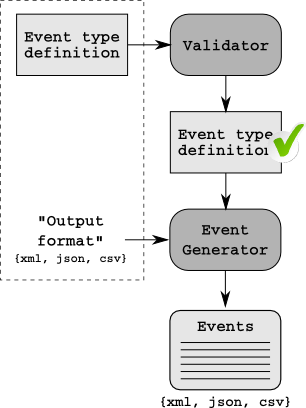
\includegraphics[scale=0.5]{./img/IoT-EGArquitecture}
  \caption[IoT-TEG Architecture]{IoT-TEG Architecture~\cite{TesisGutierrez2017,Gutierrez2017}.}
  \label{fig:IoT-EGArquitecture}
\end{figure}

Previous studies suggested there were no differences in testing effectiveness between using events
generated by IoT-TEG, or events recorded from various case studies~\cite{TesisGutierrez2017,Gutierrez2017}.
Moreover, thanks to its implementation, IoT-TEG can be used to do different types of tests: functional,
negative, integration, stress, etc; in deed an example of its usability can be found 
in~\cite{TesisGutierrez2017,gutierrez2018}, where IoT-TEG has been used to apply mutation 
testing~\cite{jia2011}. These results confirm IoT-TEG can 
simulate many types of events occurring in any type of applications,
it can provide different types of tests
and it can solve the main challenges developers face when they test event-processing programs: lack of data 
for testing, needing specific values for the events, and needing the source to generate the events.

For the sake of clarity, Example~\ref{eventTypeDef} shows an event type
definition that could be used to test the queries of Example~\ref{EPLqueries}.

\begin{lstlisting}[basicstyle=\ttfamily\footnotesize,language=XML,caption=Event type definition example,label=eventTypeDef]
<?xml version="1.0" encoding="UTF-8"?>
<event_type name="TemperatureEvent">
  <block name="feeds" repeat="150">
    <field name="created_at" quotes="true" type="ComplexType">
     <attribute type="Date" format="yy-MM-dd"></attribute>
     <attribute type="String" format="T"></attribute>
     <attribute type="Time" format="hh:mm"></attribute>
    </field>
    <field name="entry_id" quotes="false" type="Integer" 
    min="0" max="10000"></field>
    <field name="temperature" quotes="false" type="Float" 
    min="0" max="500" precision="1"></field>
  </block>
</event_type>
\end{lstlisting}

The defined event type contains three properties: \texttt{created\_at},
\texttt{entry\_id} and \texttt{temperature}. These properties are defined as
fields in the event type definition. The \texttt{created\_at} field is complex
type and \texttt{entry\_id} and \texttt{temperature} are simple types. 
%The
%property that is evaluated in the Example~\ref{eventTypeDef} queries is
%\texttt{temperature}.

% Apart from the mentioned challenges that IoT-TEG solves in order to test 
% event-processing programs, it incorporates a specific functionality
% for testing programs than use EPL of EsperTech. This functionality helps to 
% automatically generate events with specific values in accordance with the 
% program which will process them. IoT-TEG analyses the Esper EPL queries and 
% generates events depending on the logical and relational operations. Following 
% the Example~\ref{EPLqueries}, the generated events will have their temperature 
% higher than 400.

\section{Prototype}
\label{sec:basicprototype}

\subsection{Architecture}
\label{sub:basicprototypearchitecture}

The system architecture is an important part to provide a precise and reliable fall-analysis. 
Additionally, the aspect of patient compliance should be taken into consideration, because the 
system should be developed not only from the developer point of view, but it should be accepted 
by the patients. An important requirement of the elderly is that the hardware design should 
facilitate the freedom of movement. Furthermore, the system should guarantee a reliable 
functionality and a redundancy to protect the wearable system against
a total system failure. J{\"a}ms{\"a} et al.~\cite{jamsa2014fall} state that the best
position of an accelerometer is near the waist.
With reference to these aspects a BAN in form of a belt was developed which 
includes a five sensor nodes which is based on ZigBee/IEEE 802.15.4\footnote{\url{http://www.zigbee.org/}}.

\begin{figure}[!ht]
  \centering
  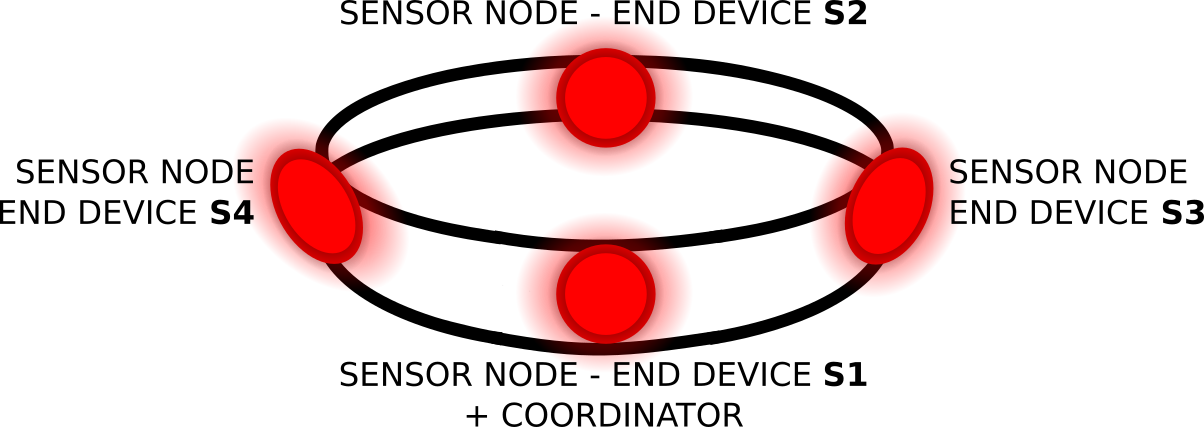
\includegraphics[scale=0.25]{./img/belt}
  \caption[Fall-detection belt]{Fall-detection belt~\cite{LaBlunda.2016,LaBlunda.2016b}}
  \label{fig:belt}
\end{figure}

Four of the sensor nodes are acting as end-devices (S1-S4) and the other node as a coordinator. 
The end-devices have attached an accelerometer and gyroscope which acquire continuously sensor 
data and is sent wirelessly to the coordinator using the ZigBee protocol. The data is sent in the following format:
 \begin{center}
  $|\alpha|, \omega_{x}, \omega_{y}, \omega_{z}$
 \end{center}
\begin{itemize}
  \item $|\alpha| \rightarrow$ This value
    represents the acceleration magnitude which is calculated  
  by equation (\ref{eq:acel}), see Section~\ref{subsec:analysis}. This value is a reference for impact detection. 
  The value's unit is m/s$^2$.
  \item $\omega_{x} \rightarrow$ represents the angular velocity in X direction. The value's unit is 
  degree per second (dps).
  \item $\omega_{y} \rightarrow$ represents the angular velocity in Y direction. The value's unit is 
  degree per second (dps).
  \item $\omega_{z} \rightarrow$ represents the angular velocity in Z direction. The value's unit is degree per second (dps).
\end{itemize}
The coordinator receives the incoming data and it has the function to evaluate the patient's status.

The proposed positioning of sensors in the belt architecture was
designed mainly for two reasons. The first reason  
reflects the requirement of a safety critical system to which the
fall-detection prototype belongs. The reliability  
of the system must be ensured, in case one of the nodes fails. Using
the architecture shown above (see Figure \ref{fig:belt}),  
a mirroring of the opposing sensors is achieved with identical sensor values, only with different signs. 
In case a node fails, the opposite value can be taken as a reference to detect a possible fall. The other reason for 
applying the proposed architecture is that it significantly improves the accuracy of our system. Taking into 
consideration the following illustration the proposed belt architecture
(see Figure \ref{fig:axisreference}) facilitates the recognition of several fall-types.

\begin{figure}[!ht]
  \centering
  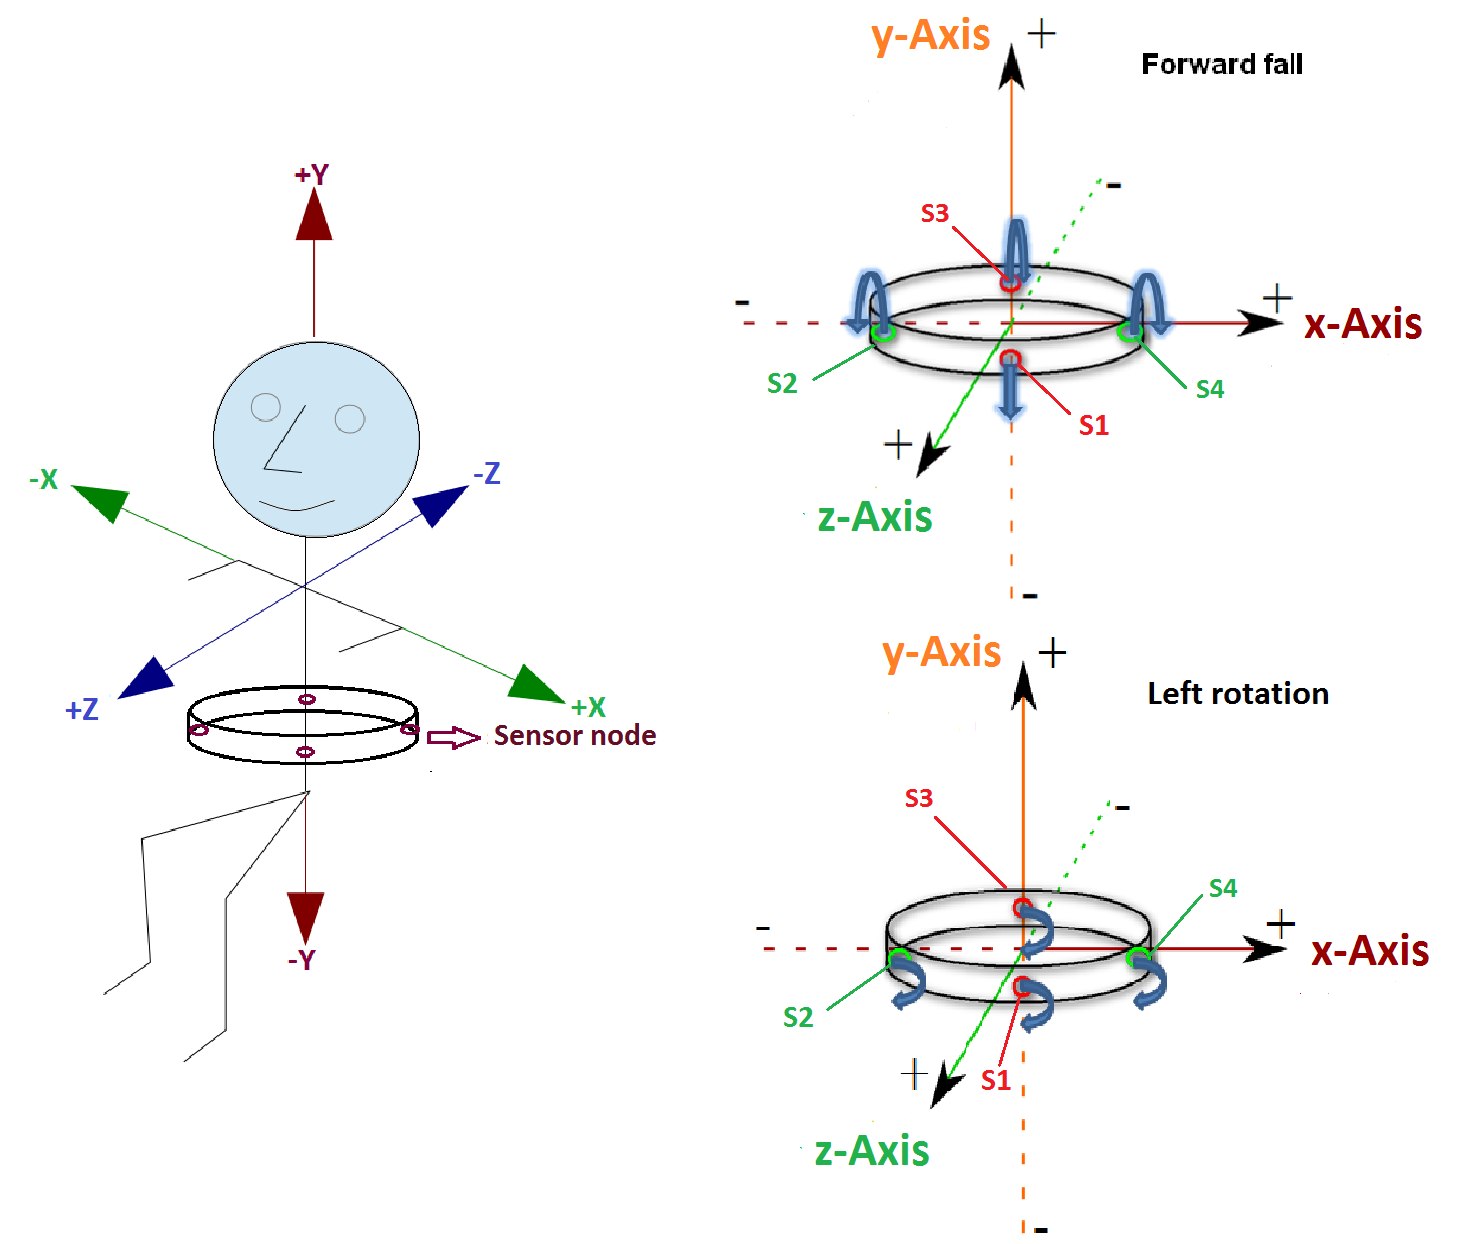
\includegraphics[scale=0.2]{./img/axis}
  \caption[Three axis reference draft]{Three axis reference draft \cite{LaBlunda.2016b,LuigiMasterThesis}}
  \label{fig:axisreference}
\end{figure}

The special positioning of the nodes on the belt results in a more precise fall-characterisation. Considering 
the event that a person does a left rotation and suffers a frontal impact to the ground (forward fall), 
the gyroscope information (single values $\omega_{i}, i \in \{x,y,z\}$) could be used for the detection of rotation and the 
acceleration magnitude $|\alpha|$ to detect the impact to the ground, see equation (\ref{eq:acel}), Section~\ref{subsec:analysis}.

To test the system's accuracy different fall-types were reproduced with several test people. A 
test procedure based on Li et al.~\cite{Li2009} and Pannurat et al.~\cite{Pannurat2014} was developed which includes 
several motions and fall-types which are typical in nursing homes and hospitals.

Taking into account the architecture of the prototype and the rule to define a fall, see Equation (\ref{eq:acel}), 
the EPL of EsperTech pattern to define the fall situation is the one shown in the Example~\ref{FallPattern}.

\begin{lstlisting}[basicstyle=\ttfamily\footnotesize,language=SQL,caption=Fall pattern,label=FallPattern]
  select a1.accelS1, a2.accelS1, a1.accelS2, a2.accelS2 from 
   pattern [every(a1=BodyEvent(a1.accelS1 <= 9.81) -> 
   a2=BodyEvent(a2.accelS1 -a1.accelS1 >= 9.81 and 
   a1.PersonID = a2.PersonID) 
   where timer:within(1sec)) or every 
   (a1=BodyEvent(a1.accelS2 <= 9.81)
   -> a2=BodyEvent(a2.accelS2-a1.accelS2 >= 9.81
   and a1.PersonID = a2.PersonID) where timer:within(1sec))];
 \end{lstlisting}

The illustrated EPL query is based on the physical principle depicted in 
Figure \ref{fig:grafica}. Important to know is that for EPL query two nodes 
were used (one frontal sensor node \& one lateral sensor node) to apply the 
fall-detection, but in future this query will be extended to four sensor nodes. 
The four node architecture (see Figure \ref{fig:belt}) is currently only used 
for redundancy purposes. With the \textit{select} statement the event properties 
are selected to create a pattern for fall-detection. In the given example the
following event properties are selected:

\begin{itemize}
 \item \texttt{a1.accelS1}: starting acceleration value of node 1.
 \item \texttt{a2.accelS1}: subsequent acceleration value of node 1.
 \item \texttt{a1.accelS2}: starting acceleration value of node 2.
 \item \texttt{a2.accelS2}: subsequent acceleration value of node 2.
\end{itemize}

Taking into consideration the selected event properties the query checks if the 
starting acceleration of sensor node 1 is $<=$ 9.81 m/s$^2$ which means the person 
is in a stationary position in which the earth's gravity of 1g (9,81 m/$s^2$) acts 
on the body. Additionally the subsequent acceleration of the first node checks if the 
subtraction of the subsequent acceleration and the first acceleration within a 
time window of 1 second is $>=$ 9.81 m/$s^2$ which means that the patient has 
suffered an impact to the ground. Using the \textit{OR} disjunction the second 
sensor node can be added and the statement is able to detect a fall in case one 
of the nodes matches the EPL query and the values of the acceleration correspond 
to the same person. 
 
\subsection{Fall simulation test events} 

The fall to generate the test events has been selected from~\cite{Li2009,Pannurat2014}. 
The fall type consists on rolling in the bed and fall (RBF). In this study we have used a 
healthy subject, and we have recorded falls with all possible realism while also
trying to avoid risks. The person has been doing RBF type falls for a period of 2 minutes. The analysed 
data and videos can be found in ~\cite{FallRepo}. In the following lines the steps to simulate 
the fall with the generated events are described, theses steps are very similar to the 
ones followed by~\cite{colladomachine,colladoTriaxal}:

\subsubsection*{1. Study of the values} Given that the sensor 1 is the one that suffers the
impact, its acceleration values are the first to be analysed. Figure~\ref{fig:Sensor1Sombras} 
shows the acceleration data from sensor 1 while the person was falling. The goal is to study 
the acceleration behaviour during a fall in order to generate test events, so the acceleration 
values are normalised ($N(m/s^2)$). The normalised acceleration is
shown on the Y-axis, and the 
time in milliseconds (ms) on the X-axis.

While performing the data analysis, it has to be taken into account that the values suffer 
alterations because several factors: the person's movement, the person bouncing against something 
(floor, wall, etc), the collocation of the sensors to the original position after a fall, 
sensor pressure because of an impact or the person is laying over it, etc.

 \begin{figure*}[!ht]
  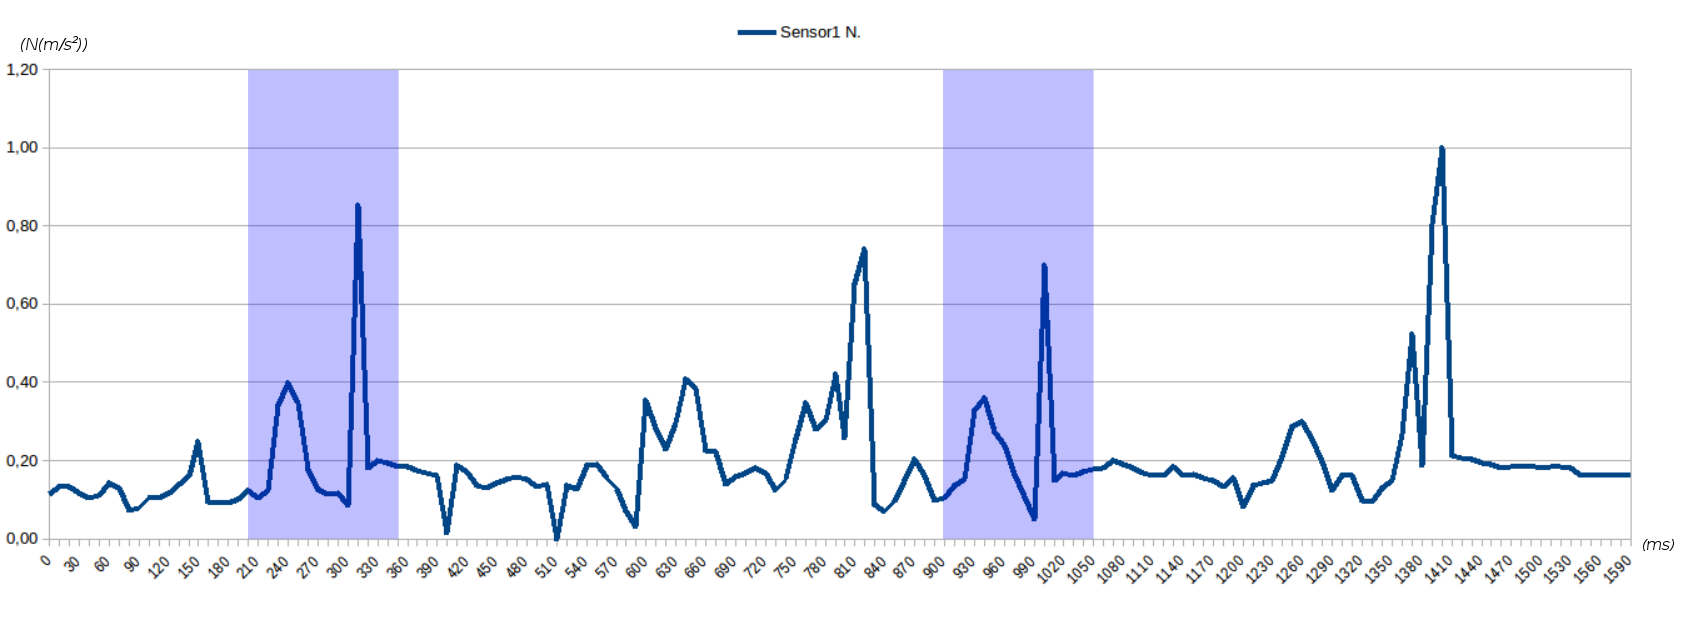
\includegraphics[scale=0.255]{img/Sensor1Sombras}
  \caption[Sensor 1 acceleration]{Sensor 1 acceleration.}
  \label{fig:Sensor1Sombras}
\end{figure*}

\subsubsection*{2. Fall identification and analysis} After the previous study, the peaks of the acceleration are identified. 
These peaks, or maximum values, are when the sensor suffers the impact. Because the mentioned noise, two ranges of the obtained 
values are extracted in order to analyse data properly. Please, see the highlighted parts in Figure~\ref{fig:Sensor1Sombras};
with respect to the X-axis $[210, 360]$ (Fall 1) and $[900, 1050]$ (Fall 2). The range of extracted values are a set of data that 
happen in less than a time window of 1 second, to meet the fact described in~\cite{Luder2009}. So as to compare both RBF falls
the acceleration values are normalised according to their impact value. The Table~\ref{tabla:RBF} 
shows the values to analyse where the impact value is highlighted with colour green.

\begin{table}[!ht]
 \centering
 \begin{tabular}{*{5}{r}}
   \centering
\begin{tabularx}{9cm}{@{}ccc|ccc@{}}
  \toprule
  \multicolumn{1}{p{0.65cm}}{\centering \textsc{Time} \\ ($s.ms$)} & \multicolumn{1}{p{0.65cm}}{\centering \textsc{Accel.} \\ ($m/s^2$)} & \multicolumn{1}{p{2cm}}{\centering \textsc{N. Accel.} \\ ($N(m/s^2)$)} & \multicolumn{1}{p{0.65cm}}{\centering \textsc{Time} \\ ($s.ms$)} & \multicolumn{1}{p{0.65cm}}{\centering \textsc{Accel.} \\ ($m/s^2$)}& \multicolumn{1}{p{2cm}}{\centering \textsc{N. Accel.} \\ ($N(m/s^2)$)} \\
  \midrule
0 & 6,29 & 0,02 & 0 & 5,98 & 0,08\\
10 & 7,57 & 0,05 & 10 & 6,31 & 0,08\\
20 & 20,7 & 0,33 & 20 & 8,2 & 0,13\\
30 & 24,07 & {\setlength{\fboxsep}{0pt}\colorbox{blue}{0,41}} & 30 & 9,21 & 0,16\\
40 & 21,01 & 0,34 & 40 & 19,92 & 0,43\\
50 & 10,81 & 0,12 & 50 & 21,8 & {\setlength{\fboxsep}{0pt}\colorbox{blue}{0,48}}\\
60 & 7,71 & 0,05 & 60 & 16,52 & 0,34\\
70 & 6,87 & 0,04 & 70 & 14,41 & 0,29\\
80 & 7,06 & 0,04 & 80 & 9,97 & 0,18\\
90 & 5,23 & {\setlength{\fboxsep}{0pt}\colorbox{bananayellow}{0,00}} & 90 & 6,54 & 0,09\\
100 & 51,58 & {\setlength{\fboxsep}{0pt}\colorbox{applegreen}{1,00}} & 100 & 3,01 & {\setlength{\fboxsep}{0pt}\colorbox{bananayellow}{0,00}}\\
110 & 11,01 & 0,12 & 110 & 42,34 & {\setlength{\fboxsep}{0pt}\colorbox{applegreen}{1,00}}\\
120 & 12,12 & 0,15 & 120 & 8,96 & 0,15\\
130 & 11,77 & 0,14 & 130 & 10,14 & 0,18\\
140 & 11,26 & 0,13 & 140 & 9,81 & 0,17\\
150 & 11,16 & 0,13 & 150 & 10,45 & 0,19\\
  \bottomrule
\end{tabularx}






 \end{tabular}
 \caption{RBF fall acceleration, fall (range) 1 and fall (range) 2}%
 \label{tabla:RBF}
\end{table}

The obtained data do not have a timestamp, so given that every 10 milliseconds the system sends the data, we have
divided the values according to this time. To compare the RBF falls the time in the Table~\ref{tabla:RBF} 
starts in 0 $ms$ and then increase in 10 $ms$, that is what it is shown in 
the first column of the Table. The second column shows the acceleration values ($m/s^2$) and the normalised acceleration values
are deployed in the third column ($N(m/s^2)$) according to the fall maximum value. In 
Figure~\ref{fig:Sensor1} a comparison of the normalised acceleration behaviour during the previous RBF falls is shown. 
This comparison shows a similar behaviour of the acceleration during the RBF falls.
Moreover, the acceleration in these two RBF falls follow the rule that define a fall, see Equation (\ref{eq:caida}), 
see Section~\ref{subsec:analysis}.

\begin{figure}[!ht]
  \centering
  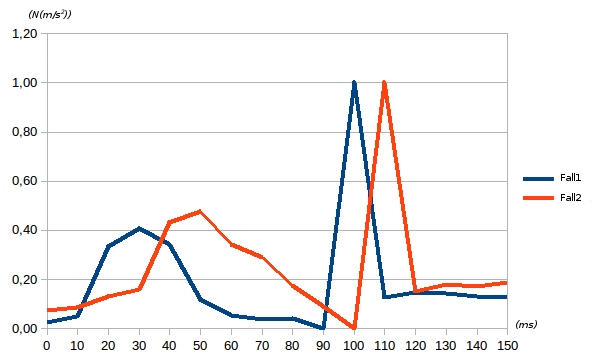
\includegraphics[scale=0.5]{img/Comparativa}
  \caption[Acceleration comparative]{Acceleration comparative.}
  \label{fig:Sensor1}
\end{figure}

The goal is to simulate this type of fall with events to test the IoT system, so we have to analyse the values of 
the acceleration before and after the impact. Taking into account that the maximum value of the acceleration is 
when the impact occurs ($\alpha_{max}$), the acceleration behaviour during a RBF fall consists on:
\begin{enumerate}
 \item from a value less than the half of $\alpha_{max}$, the acceleration value increases to obtain a value in the range:
  \begin{center}
  $[\alpha_{max}/2 - 0.5, \alpha_{max}/2 + 0.5]$
  \end{center}
 The person is rolling on the bed.
 \item if the acceleration obtains a value in the previous range, its value decreases until the minimum value $\alpha_{min}$.
 The person is falling, a free fall.
 \item the acceleration value goes from the minimum value $\alpha_{min}$ to the maximum value $\alpha_{max}$. The person
 suffers the impact.
 \item the acceleration value is established with values around the half of $\alpha_{max}$. The person is laying on the floor. 
\end{enumerate}

The same analysis process has been done to the rest of sensors, and the behaviour of the acceleration of all of them 
follows the same pattern.

Taking into account the architecture of the prototype and the previous rules to define a RBF fall, the EPL of EsperTech
pattern to the define a RBF fall is the one shown in the Example~\ref{RBFpattern}.

%include mathscape to use use the option mathescape for your environment which gives you the ability to use the normal latex behavior of the $-signs
\begin{lstlisting}[basicstyle=\ttfamily\footnotesize,language=SQL, mathescape,caption=RBF pattern,label=RBFpattern]
select a1.accelS1, a2.accelS1, a3.accelS1, a4.accelS1 from 
pattern[every(a1 = BodyEvent(a1.accelS1 <= 9.81) -> 
a2 = BodyEvent(a2.accelS1 - a1.accelS1 >= 9.81) ->
a3 = BodyEvent(a3.accelS1 < 9.81) ->
a4 = BodyEvent(a4.accelS1 - a3.accelS1 >= 9.81 
and a2.accelS1 = a4.accelS1 / 2 $\pm$ 0.5) where timer:within(1sec))];
\end{lstlisting}

The displayed EPL query depicts a recognition pattern which could be used to detect the rolling out of bed. Given that all the sensors are following the same pattern, one sensor node (S1) was used to create the query which makes it easier to understand the pattern. With the \textit{select} statement the event properties are selected to create a fall-detection pattern. In the given query the following event properties are selected:
\begin{itemize}
  \item \texttt{a1.accelS1}: starting acceleration value for stationary position (e.g. laying).
  \item \texttt{a1.accelS2}: subsequent acceleration value for rolling event.
  \item \texttt{a1.accelS3}: subsequent acceleration value for free fall event.
  \item \texttt{a1.accelS4}: subsequent acceleration value for impact detection.
\end{itemize}

Taking into consideration that the RBF fall is a complex event to detect, this event has been divided in the following phases:

\begin{itemize}
  \item Stationary phase (e.g. laying).
  \item Rolling phase.
  \item Free fall phase.
  \item Impact phase.
\end{itemize}

The EPL query first checks if the starting acceleration \texttt{a1.accelS1} is $<=$ 9.81m/$s^2$ which means that the person is laying 
on the bed (stationary position). Additionally the subsequent property is checked. If the difference between the successive 
acceleration value (\texttt{a2.accelS1}) and the previous one (\texttt{a1.accelS1}) is $>=$ 9.81 m/$s^2$ then the person has a transition to 
the rolling phase. If the person is falling after turning, the subsequent acceleration value should be $<$ 9.81 m/$s^2$ 
which means that the person is in the free fall phase. Additionally, if the difference between the current acceleration value 
(\texttt{a4.accelS1}) and the previous one (\texttt{a3.accelS1}) is $>=$ 9.81 m/$s^2$, it is an indication for a fall. So that the query 
recognises this event as a fall all these sequences should happen within a time window of 1 second.

\subsubsection*{3. To define the fall event} Once the fall acceleration behaviour has been observed, the next step is to define the 
fall event in order to generate test events with IoT-TEG~\cite{TesisGutierrez2017,Gutierrez2017}. As it was explained in 
Section~\ref{iotteg}, the event type attributes have
to be defined using the \texttt{<field>} element. The fall event contains one attribute, the acceleration, which is float, 
\texttt{type=``Float''}, and its values are not quoted, \texttt{quotes=``false''}. A new parameter in IoT-TEG has been defined as a 
consequence of the previous falls study. Given that the acceleration values follow a specific behaviour, it is necessary to include 
the \texttt{custom\_behaviour} property in the \texttt{<field>} element to define the behaviour of any event attribute; 
in this study, the acceleration. In the \texttt{custom\_behaviour} property the path to the file that includes the behaviour of the 
event attribute has to be written. The Example~\ref{FallEvent} shows the complete fall event definition (FallEventType).

\begin{lstlisting}[basicstyle=\ttfamily\footnotesize,language=XML,caption={Fall event type definition},label=FallEvent]
<?xml version="1.0" encoding="UTF-8"?>
<event name="FallEventType">
<block name="feeds" repeat="100">
 <field name="acceleration" quotes="false" type="Float" 
 custom_behaviour="/Path/To/Rule/File"></field>
</block>
</event>
\end{lstlisting}

IoT-TEG includes a new functionality, which has been implemented to simulate the desired behaviour of an 
event attribute with a \texttt{custom\_behaviour} property in its event type definition. This functionality 
allows to generate values of the event attribute following a behaviour
that the IoT-TEG user has described in a file.
In order to explain how the user has to define the desired behaviour of an event attribute, we are going
to use the RBF fall behaviour rules (see Example~\ref{RBFFallRules}). In a XML file the number of simulations has to be
indicated, the events involved in a simulation will be calculated according to the total number of events
to generate and the desired simulations. For example, if the number of test events to generate is 100, 
the number indicated in the event type definition file, \texttt{repeat="100"}, and the number of desired 
simulations is 5, \texttt{simulations="5"}, the number indicated in the behaviour rules definition file, 
the number of events involved to simulate the behaviour is 20. In the RBF fall example, the user asks to 
generate 100 test events and 5 falls (simulations), so 20 events will be used to define a RBF fall.

Variables can be defined if they are needed in the behaviour rules. They can be defined in the file where
the behaviour rules are included using the \texttt{<variables>} tags. To define them a name and a value 
have to be given to the variables. The value can be defined as a fixed value with the \texttt{value} 
property, or using a range with the \texttt{min} and \texttt{max} properties. Moreover, in some variables
are involved in the value of another variables; this is indicated using the variable with an specific 
format \texttt{\$(variable)}, see Example~\ref{RBFFallRules}. In addition, arithmetic operations can be 
done in the definition of the variable values. Let us see how using them in the RBF fall example. To 
define the acceleration behaviour during a RBF fall three variables are defined: \texttt{Roll}, 
\texttt{Fall} and \texttt{Impact}. \texttt{Impact} will be the maximum value $\alpha_{max}$, 
\texttt{Fall} will be the minimum value $\alpha_{min}$ and the \texttt{Roll} variable is defined by a 
range where the acceleration value will be obtained according to the \texttt{Impact} value. In order to
obtain a low value, a range between 0 and the fifth part of \texttt{Roll} is assigned to the \texttt{Fall} 
variable.

Once the variables are defined, the \texttt{<rules>} tags are used to define the rules. A \texttt{weight}
must be assigned to each one to calculate the number of events to generate for each rule for each simulation.
Following the example and the assigned \texttt{weight} in Example~\ref{RBFFallRules}, if 20 events simulate 
a RBF fall $20 * 0,25 = 5$ events will be generated for the first rule, another 5 events for the second rule,
1 event for the third rule, and the remained events for the fourth rule. We have to assign zero to the weight
\texttt{weight="0"} to indicate how the remained events have to be generated.

To define the rules, \texttt{min}, \texttt{max} and \texttt{value} properties can be used as well as the arithmetic 
operations and the references to another variables. Moreover, the \texttt{sequence} property can be used to obtain
values lower or higher than the one generated previously. The \texttt{sequence} property values are \texttt{inc}, 
to increase the value, or \texttt{dec}, to decrease the value.

Thanks to the included properties and parameters in the IoT-TEG new functionality, the desired behaviour rules can
be defined. In the RBF fall rules, the involved event attribute is the acceleration, and its behaviour during the 
fall is defined by four rules; in the first rule the acceleration value increases to a value close or equal to \texttt{Roll},
in the second rule the acceleration value decreases to a value close or equal to \texttt{Fall}, in the third rule the 
acceleration value is equal to \texttt{Impact}, it obtains the highest value and in the fourth rule the acceleration value
is established in a range which is lower than \texttt{Roll}.

\begin{lstlisting}[basicstyle=\ttfamily\footnotesize,language=XML,caption={Rules to define a RBF fall},label=RBFFallRules]
  <?xml version="1.0" encoding="UTF-8"?>
  <custom_conditions simulations="5">
  <variables>
   <variable name="Impact" min="40.0" max="156.96"/>
   <variable name="Roll" min="$(Impact)/2-0.5" 
    max="$(Impact)/2+0.5"/>
   <variable name="Fall" min="0.0" max="$(Roll)/5"/>
  </variables>
  <rules>
   <rule weight="0.25" min="$(Roll)/4" max="$(Roll)" 
    sequence="inc"/>
   <rule weight="0.25" min="$(Roll)" max="$(Fall)" sequence="dec"/>
   <rule weight="1" value="$(Impact)"/>
   <rule weight="0" min="$(Roll)/2-0.25" max="$(Roll)/2+0.25"/>
  </rules>
  </custom_conditions>
\end{lstlisting}

It is needed to highlight that to obtain these rules to define the behaviour of the acceleration several test
have been done. Once we obtained the desired results, test events were generated as they were necessary. The 
Figure~\ref{fig:IoTTEGRBFGeneratedEvents} shows the acceleration values of some of the generated RBF falls using
IoT-TEG and the new functionality.

\begin{figure}[!ht]
  \centering
  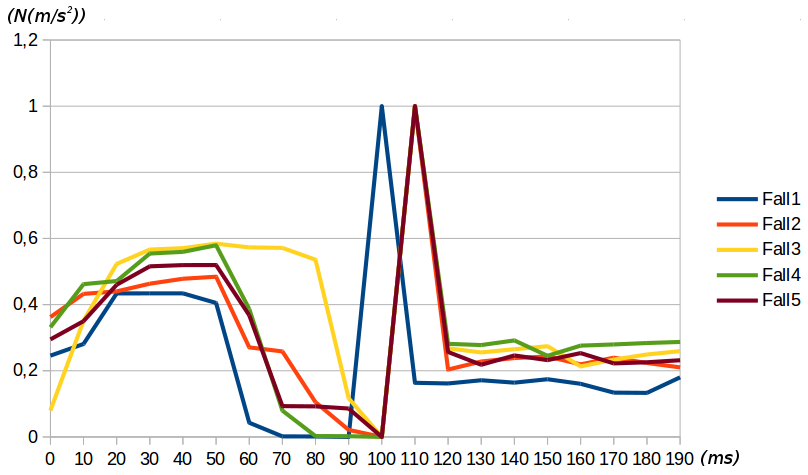
\includegraphics[scale=0.3]{img/IoTTEGRBFGeneratedEvents}
  \caption[IoT-TEG generated RBF falls]{IoT-TEG generated RBF falls.}
  \label{fig:IoTTEGRBFGeneratedEvents}
\end{figure}

The generated events which simulate RBF falls follow the pattern of the acceleration during a RBF fall.
So, these generated events can be used to test the fall detection system.

\section{Improved prototype}
\label{sec:improvedprototype}

\subsection{Architecture}
\label{sub:improvedprototypearchitecture}

Taking into consideration the architecture of the prototype described in the previous 
section significant improvements were done. The improved hardware architecture is also 
based on four sensor nodes (S1-S4), but with the following significant innovations:

\begin{itemize}
 \item A new hardware platform which is based on Arduino Primo Core~\cite{Arduino2018}. 
 This micro-controller provides built-in sensors and a Bluetooth Low Energy (BLE) 
 interface for wireless data transmission. This satisfies the
 requiremnent of patient compliance
 which includes the mobility of movement.
 \item A different power supply mode is used for the improved prototype. Instead of 
 using the Lithium Polymer (LIPO) batteries, the Arduino Primo Core is supplied by a 
 coin cell. This is an important aspect due to the fact, that exposing the LIPO-batteries 
 to permanent shocks will damage them and drastically shorten their lifespan. 
 Additionally with the usage of coin cells, we have reached a lifespan of 2 to 3 weeks 
 without exchanging the battery.
 \item The improved Prototype is using BLE for wireless data transmission. Using BLE 
 brings the advantage to build up a communication infrastructure with the smartphone 
 to automatically inform the emergency services without any additional hardware.
 \item The dataset which is sent by the sensor nodes (S1- S4) is composed as follows 
 and includes the values unit m/$s^2$:
 \begin{center}
  \texttt{SensorID, X-Acceleration, Y-Acceleration, Z-Acceleration}
 \end{center}
 Compared to the dataset format of the previous prototype the sensor identification 
 number was added and the significantly change is that only the single axis values of 
 the accelerometer are sent. Based on the individual axis values of the accelerometer, 
 the orientation of the person can also be determined. Assuming the person is in a standing 
 position, the x-axis corresponds to 1G ($\pm$ 9.81m/$s^2$) and the other two axes would be 
 approximately 0G. This indicates that the person is standing. As the person changes 
 position, the gravitational acceleration will occur on one of the other axis. For that 
 reason, in the improved prototype the single axis values were taken as orientation 
 reference. To detect the impact the single values were used to calculate the acceleration 
 magnitude based on Equation (\ref{eq:acel}), see Section~\ref{subsec:analysis}.
\end{itemize}

\subsection{Fall simulation test events}

The second fall to generate the test events consists on the impact of the person with 
a wall and falling on the knees and then on the chest: \textit{fall against wall} (FAW). 
In this study we have used two healthy subjects, and we have recorded falls with all 
possible realism while also trying to avoid risks. They have been doing fall test for a period 
of 2 minutes, the FAW fall type. The analysed data and videos can be found in ~\cite{FallRepo}.

In this analysis the same steps that the ones described in Section~\ref{sec:basicprototype} 
have been done:

\subsubsection*{Study of the values} Given that the sensor 1 is the one that suffers the 
impact, its acceleration values are the first to be analysed. The acceleration values have 
been normalised ($N(m/s^2)$). After the normalisation the impacts of the falls, peaks, 
have to be detected; we have considered a peak when the normalised acceleration is 
greater than 0,7 ($N(m/s^2) > 0,7$). After applying the previous rule in all the fall data 
and taking into account the alterations because the mentioned factors, the impacts are detected.

\subsubsection*{Fall identification and analysis} Once the peaks are detected, a range of values, 
including the peaks, are selected in order to analyse data properly and to study the acceleration 
behaviour during FAW fall. The range of extracted values are a set of data that happen in less 
than a time window of 1 second, to meet the fall rule of~\cite{Luder2009} described in 
Equation (\ref{eq:caida}), see Section~\ref{subsec:analysis}. The Table~\ref{tabla:FAW} shows the 
acceleration value during one FAW fall of person 1 and person 2. 

\begin{table}[!ht]
 \centering
 \begin{tabular}{*{5}{r}}
   \centering
\begin{tabularx}{9.5cm}{@{}ccc|ccc@{}}
  \toprule
  \multicolumn{1}{p{0.65cm}}{\centering \textsc{Time} \\ ($s.ms$)} & \multicolumn{1}{p{0.65cm}}{\centering \textsc{Accel.} \\ ($m/s^2$)} & \multicolumn{1}{p{2cm}}{\centering \textsc{N. Accel.} \\ ($N(m/s^2)$)} & \multicolumn{1}{p{0.65cm}}{\centering \textsc{Time} \\ ($s.ms$)} & \multicolumn{1}{p{0.65cm}}{\centering \textsc{Accel.} \\ ($m/s^2$)}& \multicolumn{1}{p{2cm}}{\centering \textsc{N. Accel.} \\ ($N(m/s^2)$)} \\
  \midrule
57.311 & 3,63 & 0,01 & 25.254 & 8,53 & 0,09 \\
57.359 & 3,43 & 0,00 & 25.303 & 10,79 & 0,19 \\
57.408 & 7,85 & 0,17 & 25.352 & 11,28 & 0,22 \\
57.506 & 10,99 & 0,30 & 25.401 & 13,83 & 0,34 \\
57.506 & 6,47 & 0,12 & 25.449 & 9,42 & 0,13 \\
57.554 & 4,61 & 0,05 & 25.503 & 8,63 & 0,09 \\
57.603 & 4,22 & 0,03 & 25.546 & 0,89 & 0,10 \\
57.651 & 22,86 & {\setlength{\fboxsep}{0pt}\colorbox{bananayellow}{0,77}} & 25.596 & 8,04 & 0,07 \\
57.700 & 28,84 & {\setlength{\fboxsep}{0pt}\colorbox{bananayellow}{1,00}} & 25.645 & 13,93 & 0,35 \\
57.749 & 21,78 & {\setlength{\fboxsep}{0pt}\colorbox{bananayellow}{0,72}} & 25.693 & 22,7 & {\setlength{\fboxsep}{0pt}\colorbox{bananayellow}{0,76}} \\
57.800 & 9,03 & 0,22 & 25.742 & 10,59 & 0,19 \\
57.846 & 10,79 & 0,29 & 25.791 & 8,63 & 0,09 \\
57.900 & 10,79 & 0,29 & 25.841 & 8,34 & 0,08 \\
57.944 & 9,32 & 0,23 & 25.888 & 6,67 & 0,00 \\
57.996 & 13,15 & 0,38 & 25.937 & 17,46 & 0,51 \\
58.042 & 20,99 & 0,69 & 25.986 & 27,76 & {\setlength{\fboxsep}{0pt}\colorbox{bananayellow}{1,00}} \\
58.186 & 28,25 & {\setlength{\fboxsep}{0pt}\colorbox{bananayellow}{0,98}} & 26.082 & 11,58 & 0,23 \\
58.188 & 27,47 & {\setlength{\fboxsep}{0pt}\colorbox{bananayellow}{0,95}} & 26.084 & 11,38 & 0,22 \\
58.240 & 10 & 0,26 & 26.134 & 10,5 & 0,18 \\
58.286 & 10,99 & 0,30 & 26.181 & 8,83 & 0,10 \\
58.334 & 11,67 & 0,33 & 26.230 & 12,75 & 0,29 \\
  \bottomrule
\end{tabularx}


 \end{tabular}
 \caption{FAW fall acceleration, person 1 and 2}%
 \label{tabla:FAW}
\end{table}

The first and fourth columns of the Table~\ref{tabla:FAW} represent
the seconds ($s$) and milliseconds 
($ms$) when the acceleration was measured. The second and fifth columns show the acceleration 
values ($m/s^2$) and in the third and sixth columns are deployed the normalised acceleration values 
($N(m/s^2)$) according to the fall maximum value. In Figure~\ref{fig:FAWcomparison} a comparison 
of the normalised acceleration behaviour during the previous FAW falls of person 1 and person 2 is 
shown. These comparisons show a similar behaviour of the acceleration during the FAW fall.

\begin{figure}[!ht]
  \centering
  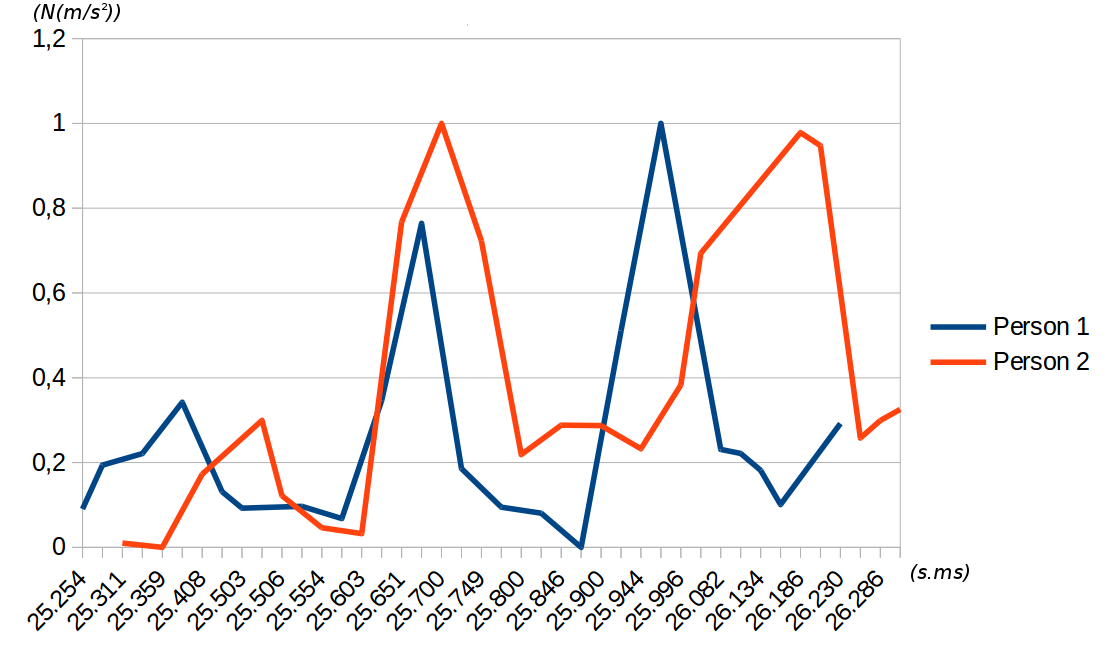
\includegraphics[scale=0.2]{img/TwoFallsComparative.png}
  \caption[Acceleration during FAW fall]{Acceleration comparison during FAW fall.}
  \label{fig:FAWcomparison}
\end{figure}

For the FAW, we have decided to define the acceleration behaviour with normalised values; so the 
normalised acceleration behaviour during the FAW consists on:
\begin{enumerate}
 \item the variation of its values while the person is walking. We have divided this rule in two rules:
 \begin{enumerate}
  \item The normalised acceleration values increase in a range [0, 0.35].
  \item The normalised acceleration values decrease in a range [0, 0.35].
 \end{enumerate}
 \item as a consequence of the impact of the person against a wall, the acceleration normalised value 
 has to be greater than 0.7.
 \item the normalised acceleration values decreases to a range [0, 0.35]. The values of the acceleration are 
 in the mentioned range depending on the size of the person; the larger person results in a longer range 
 and if the person retains a position prior to a fall thanks to the wall. Moreover, a subtle peak could 
 appear as a consequence of a rebound.
 \item a second impact happens when the person hit the ground, the acceleration normalised values has to 
 be greater than 0.7.
 \item finally, the person is laying on the ground and the normalised acceleration value decreases. The 
 values of the acceleration are between [0.10, 0.35] and no subtle peaks appear. 
\end{enumerate}

The same analysis process has been done to the rest of sensors, and the behaviour of the acceleration of all of 
them follows the same pattern.

Taking into account the architecture of the prototype and the previous rules to define a FAW fall, the EPL of EsperTech
pattern to the define a FAW fall is the one shown in the Example~\ref{FAWpattern}.

\begin{lstlisting}[basicstyle=\ttfamily\footnotesize,language=SQL, mathescape,caption=FAW pattern,label=FAWpattern]
select a1.accelS1, a2.accelS1, a3.accelS1, a4.accelS1, a5.accelS1 
from pattern[every(a1 = BodyEvent(a1.accelS1 >= 9.81) -> 
a2 = BodyEvent(a2.accelS1 < 9.81) ->
a3 = BodyEvent(a3.accelS1 - a2.accelS1 >= 9.81) ->
a4 = BodyEvent(a4.accelS1 < 9.81) ->
a5 = BodyEvent(a5.accelS1 - a4.accelS1 >= 9.81) 
where timer:within(1sec))];
\end{lstlisting}

Considering the above EPL query, the following event properties are selected for the recognition of the FAW fall:

\begin{itemize}
  \item \texttt{a1.accelS1}: starting acceleration value for dynamic postures (e.g. walking).
  \item \texttt{a2.accelS1}: successive acceleration value for free fall before wall impact.
  \item \texttt{a3.accelS1}: subsequent acceleration value for wall impact.
  \item \texttt{a4.accelS1}: successive acceleration value for free fall event.
  \item \texttt{a5.accelS1}: subsequent acceleration value for impact to the ground.
\end{itemize}

This event has been divided in the following phases:
\begin{itemize}
  \item Dynamic phase (e.g. walking).
  \item Free fall to wall phase.
  \item Wall impact phase.
  \item Free fall phase.
  \item Impact phase.
\end{itemize}

The EPL query checks if the starting acceleration \texttt{a1.accelS1} is $>=$ 9.81 m/$s^2$ which means that the person is walking. 
The next acceleration value (\texttt{a2.accelS1}) is used to detect the free fall phase to the wall. If \texttt{a2.accelS1} 
is $<$ 9.81 m/$s^2$ it indicates that the person is falling against the fall. Additionally if the difference between 
the current acceleration value (\texttt{a3.accelS1}) and the previous acceleration value (\texttt{a2.accelS1}) is $>=$ 9.81 m/$s^2$ 
it indicates the impact against a wall. After that the person suffered the impact against a wall the upcoming 
acceleration value (\texttt{a4.accelS1}) should be less than 9.81 m/$s^2$. This indicates that the person is falling to 
the ground. If the difference between the successive value (\texttt{a5.accelS1}) and the previous value (\texttt{a4.accelS1}) 
is $>=$ 9.81 m/$s^2$ it means that the person has suffered an impact to the ground. To classify this event as 
a FAW fall this pattern flow should happen within a time window of 1 second.

\subsubsection*{To define the fall event} Once the fall acceleration behaviour has been observed, the next step is to define the 
fall event in order to generate test events with IoT-TEG~\cite{TesisGutierrez2017,Gutierrez2017}. Given that the involved event 
attribute in this fall is the acceleration, the Example~\ref{FallEvent} in Section~\ref{sec:basicprototype} can be used to define 
the fall event (FallEventType). The rules to define the behaviour of the acceleration in this type of fall is shown in 
Example~\ref{FAWFallRules}.

\begin{lstlisting}[basicstyle=\ttfamily\footnotesize,language=XML,caption={Rules to define a FAW fall},label=FAWFallRules]
  <?xml version="1.0" encoding="UTF-8"?>
  <custom_conditions simulations="5">
  <variables>
   <variable name="Base" value="9.81"/>
   <variable name="ImpactWall" min="$(Base)+$(Base)*0.7" 
    max="$(Base)*3"/>
   <variable name="Impact" min="$(Base)+$(Base)*0.7" 
    max="$(Base)*3"/>
  </variables>
  <rules>
   <rule weight="0.25" min="0" max="$(ImpactWall)*0.35" 
    sequence="inc"/>
   <rule weight="0.25" min="0" max="$(ImpactWall)*0.35" 
    sequence="dec"/>
   <rule weight="1" value="$(ImpactWall)"/>
   <rule weight="0.25" min="0" max="$(Impact)*0.35"/>
   <rule weight="1" value="$(Impact)"/>
   <rule weight="0" min="$(Base)+$(Base)*0.10"
    max="$(Impact)*0.35"/>
  </rules>
  </custom_conditions>
\end{lstlisting}

To define the acceleration behaviour during a FAW fall three variables are defined: \texttt{Base}, 
\texttt{ImpactWall} and \texttt{Impact}. Given that the acceleration behaviour during a FAW fall has
been according to the normalised values, the variables and rules have been defined according to 
that analysis. The acceleration value in a stationary position is a variable depending on the person, so 
we have considered the established value, $1g\approx9.81m/s^{2}$. That is the fixed value of the 
\texttt{Base} variable. To determine the values of the impacts, we have taken into account that the 
normalised value have to be $> 0,7$. So, to ensure that the impacts, \texttt{ImpactWall} and 
\texttt{Impact}, have a value meeting the mentioned condition the minimum value of the impact is the 
sum of the \texttt{Base} and \texttt{Base} multiplied by \texttt{Base}$*0,7$; and the maximum value of the
impacts is $3g\approx9,81*3=$\texttt{Base}$*3$.

Once the variables are defined, the rules have to be determined. The first step is to indicate the 
\texttt{weight} for each rule in order to calculate the number of events to generate for each rule for 
each simulation. Following the simulation values the number of events to generate for each rule, according 
to the assigned weights, is: $20 * 0,25 = 5$ events will be generated for the first rule, another 5 events 
for the second rule, 1 event for the third rule, 5 events for the fourth rule, 1 event for the fifth
rule and the remained events, three events, for the sixth rule. 

Thanks to the included properties and parameters in the IoT-TEG new functionality, the desired behaviour rules that
follow the normalised acceleration values can be defined. Given that we have considered to define the FAW fall behaviour
rules according to the normalised values, the values to generate depend on the maximum value. Due to there are two 
values that can be the highest one, \texttt{ImpactWall} or \texttt{Impact}, the rules that depend on the maximum 
value contains the reference to the value, \texttt{ImpactWall} or \texttt{Impact}, according to the proximity
of the rule. For instance, the first and second FAW fall rules contain a reference to \texttt{ImpactWall}, the impact 
in the wall (third rule), which happens after the person is walking, something described in the first and the second rules.
The fourth and sixth rules contain a reference to \texttt{Impact}, the impact on the ground (fifth rule), which happen
after the person is falling and the person is laying on the floor, fourth and sixth rules.

It is important to highlight that to obtain these rules to define the behaviour of the normalised acceleration several test
have been done. Once we obtained the desired results, test events were generated as they were necessary. The 
Figure~\ref{fig:IoTTEGFAWGeneratedEvents} shows the acceleration values of some of the generated FAW falls using
IoT-TEG and the new functionality.

\begin{figure}[!ht]
  \centering
  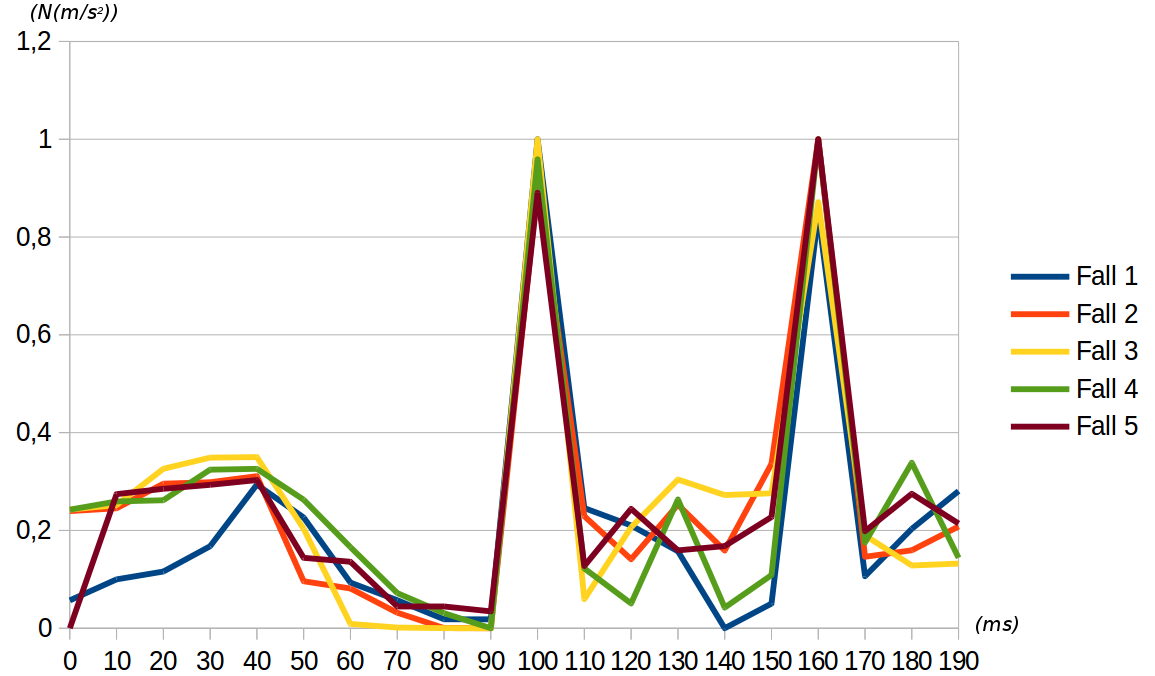
\includegraphics[scale=0.2]{img/IoTTEGFAWGeneratedEvents}
  \caption[IoT-TEG generated FAW falls]{IoT-TEG generated FAW falls.}
  \label{fig:IoTTEGFAWGeneratedEvents}
\end{figure}

The generated events which simulate FAW falls follow the pattern of the acceleration during a FAW fall.
So, these generated events can be used to test the fall detection system.

The improvements in the new prototype are encouraging. They affect not only in the way of obtaining the data, but 
also in the format and their values. The impact values from one analysis to the other are quite different, 
this is because several reasons that are described in Section~\ref{sub:detectedproblems}. The difference
of values was not a problem for IoT-TEG to define the behaviour rules and to generate the test events. That
means that the introduced functionality can be adapted to the analysed
behaviour. Moreover, it has to be emphasised that the application of the new functionality covers any event attribute which follows a behaviour;
so IoT-TEG is not limited.

\subsection{Detected problems}
\label{sub:detectedproblems}

After testing the current fall detection prototype, some problems were 
found. Moreover, some considerations will be applied in future tests.

First of all, we are going to explain the problems related to the prototype: 

\begin{itemize}
 \item Synchronisation problem of the data acquisition with $n$ sensor nodes.
 \item Fall data from the beginning should always be discarded because
   the sensors start sending data at different times. The
   Table~\ref{tabla:Synchro} will be used to explain the problem. Let
   us say  
 that in ``fall 1'', there are more than 30 values that define the fall, and later in ``fall 3'', there are 
 12 values that define the fall. So, in order to analyse the falls and compare the acceleration behaviour, it is 
 difficult to work with that information. A comparison of two FAW falls with the synchronisation problem is shown
 in Figure~\ref{fig:synchronisation1}; the sensor 1 acceleration values for the first FAW fall are coloured in blue and the
 sensor 1 acceleration values for the second FAW fall are coloured in red. The first fall is one fall from the beginning
 of the simulation, and the second one is from the middle of the simulation.
 
 \begin{table}[!ht]
 \centering
 \begin{tabular}{*{5}{r}}
   \centering
\begin{tabularx}{8cm}{@{}ccc|ccc@{}}
  \toprule
  \multicolumn{1}{p{0.65cm}}{\centering \textsc{Time} \\ ($s.ms$)}  &  \multicolumn{1}{p{0.65cm}}{\centering \textsc{Accel.} \\ ($m/s^2$)}  &  \multicolumn{1}{p{1.5cm}}{\centering \textsc{N. Accel.} \\ ($N(m/s^2)$)}  &  \multicolumn{1}{p{0.65cm}}{\centering \textsc{Time} \\ ($s.ms$)}  &  \multicolumn{1}{p{0.65cm}}{\centering \textsc{Accel.} \\ ($m/s^2$)} &  \multicolumn{1}{p{1.5cm}}{\centering \textsc{N. Accel.} \\ ($N(m/s^2)$)} \\
  \midrule
25.561 & 9,81 & 0,11 & 25.546 & 8,73 & 0,1 \\
25.561 & 9,81 & 0,11 & 25.596 & 8,04 & 0,07 \\
25.562 & 11,38 & 0,17 & 25.645 & 13,93 & 0,35 \\
25.564 & 11,38 & 0,17 & 25.693 & 22,76 & 0,76 \\
25.609 & 15,11 & 0,33 & 25.742 & 10,59 & 0,19 \\
25.610 & 15,11 & 0,33 & 25.791 & 8,63 & 0,09 \\
25.610 & 15,11 & 0,33 & 25.841 & 8,34 & 0,08 \\
25.611 & 15,11 & 0,33 & 25.888 & 6,67 & 0 \\
25.612 & 31,4 & 1 & 25.937 & 17,46 & 0,51 \\
25.612 & 23,84 & 0,69 & 25.986 & 27,76 & 1 \\
25.657 & 23,84 & 0,69 & 26.082 & 11,58 & 0,23 \\
25.657 & 23,84 & 0,69 & 26.084 & 11,38 & 0,22 \\
25.658 & 23,84 & 0,69 &  &  & \\
25.659 & 23,84 & 0,69 &  &  & \\
25.660 & 9,52 & 0,10 &  &  & \\
25.660 & 9,52 & 0,10 &  &  & \\
25.706 & 9,52 & 0,10 &  &  & \\
25.706 & 9,52 & 0,10 &  &  & \\
25.707 & 9,52 & 0,10 &  &  & \\
25.707 & 9,52 & 0,10 &  &  & \\
25.708 & 23,74 & 0,69 &  &  & \\
25.709 & 23,74 & 0,69 &  &  & \\
25.756 & 23,74 & 0,69 &  &  & \\
25.756 & 23,74 & 0,69 &  &  & \\
25.757 & 27,86 & 0,85 &  &  & \\
25.758 & 27,86 & 0,85 &  &  & \\
25.758 & 9,52 & 0,1 &  &  & \\
25.759 & 9,52 & 0,1 &  &  & \\
25.760 & 9,52 & 0,1 &  &  & \\
25.804 & 7,06 & 0 &  &  & \\
25.805 & 7,06 & 0 &  &  & \\
25.805 & 7,06 & 0 &  &  & \\
25.806 & 7,06 & 0 &  &  & \\
  \bottomrule
\end{tabularx}

 \end{tabular}
 \caption{Synchronisation problem, fall 1 and fall 2}%
 \label{tabla:Synchro}
 \end{table}
 
 \begin{figure}[!ht]
  \centering
  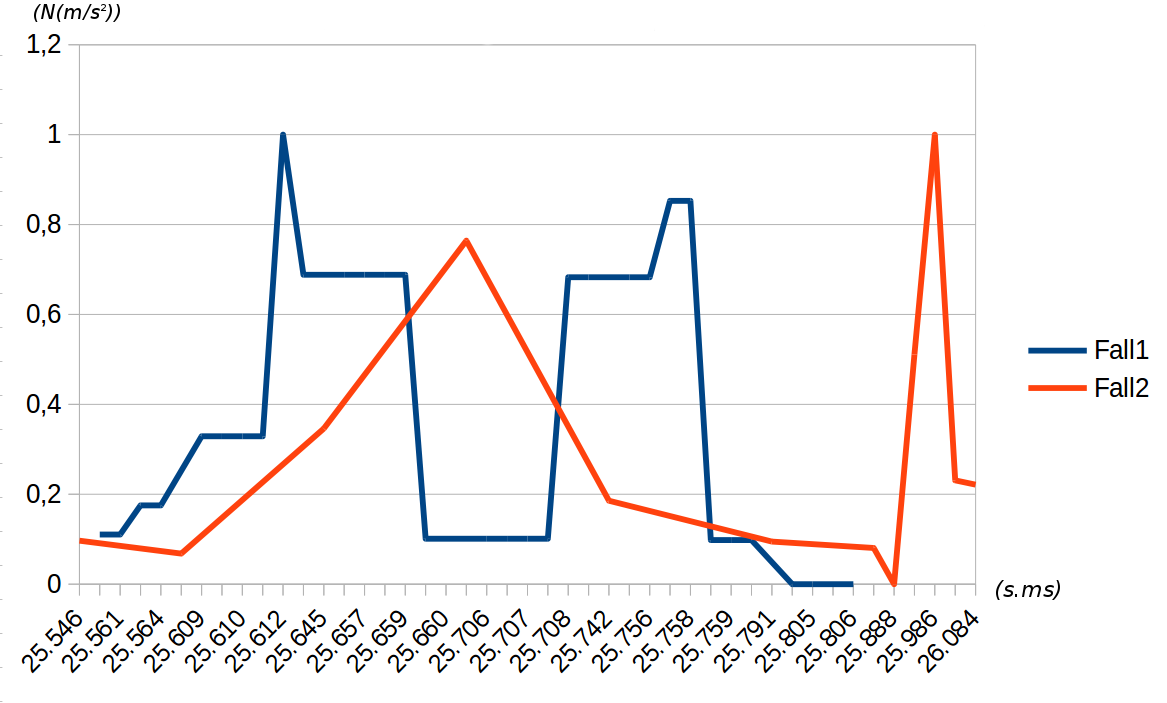
\includegraphics[scale=0.2]{img/synchronisation1.png}
  \caption[Comparison acceleration during two FAW falls]{Synchronisation problem; comparison of acceleration values during two FAW falls.}
  \label{fig:synchronisation1}
 \end{figure}
 
 The acceleration values show that in less than 250 milliseconds there are more than 30 values from ``fall 1'', and
 in more than 350 milliseconds there are 12 values from ``fall 2''. There is a lack of synchronisation not only in
 the amount of data, but also in the time.
 
 \item Some sensors transmit more data than the others, i.e. the sensors are not 
 sending the same amount of data, even sometimes there is no data. The four sensors were working while the FAW fall
 simulation, but the obtained acceleration values were from three of them, one of the sensor does not transmit data 
 in one moment of the simulation, see Figure~\ref{fig:synchronisation2}.
 
 \begin{figure}[!ht]
  \centering
  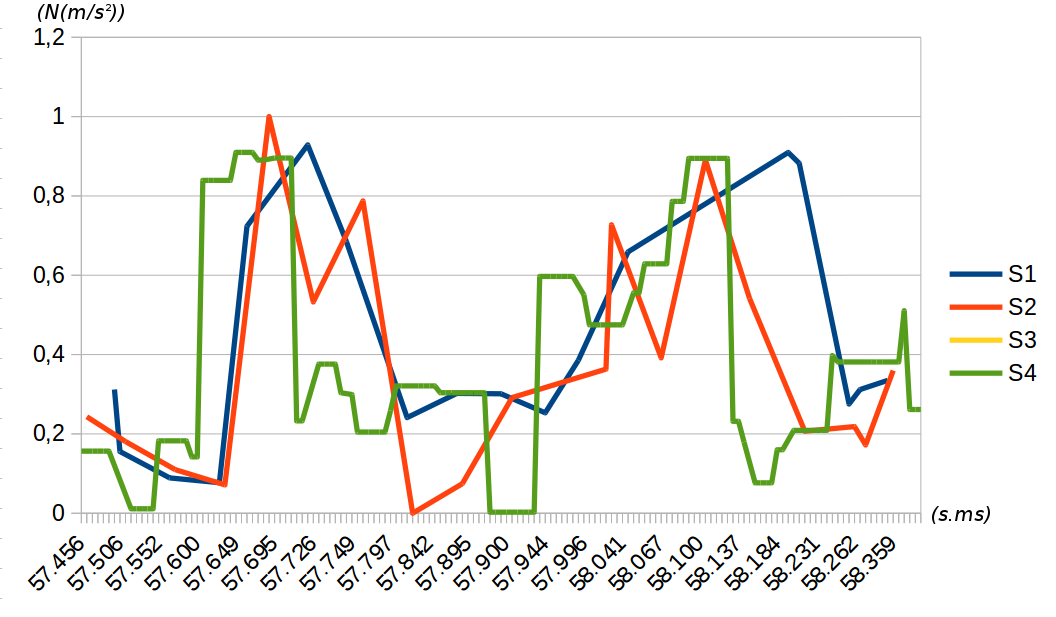
\includegraphics[scale=0.22]{img/synchronisation2.png}
  \caption[Comparison acceleration during two FAW falls]{Synchronisation problem; acceleration values from the four sensors during a FAW fall.}
  \label{fig:synchronisation2}
 \end{figure}
\end{itemize}

If we focus our attention to the hardware, the duration of the battery is also something to improve. Nowadays the 
duration of the battery is around 2 or 3 weeks, it depends on its use. If we want to use this IoT system with patients, 
specially with elderly people, or people that need special treatment, we have to increase the duration of the battery 
in order to change it as little as possible.

The analysis has revealed that while we were studying the acceleration data test, some of its values could be misinterpreted.
This is because the test person that is falling for the simulation, stands up very fast. Given that we have been cautious
in our analysis and we have been checking not only the values but also the videos and matching them, we have detected
this issue. So, in our future tests, the test person should wait at least 2 seconds laying on the floor 
after the fall for a better fall simulation. In a real situation, if a
person falls and stands up this means that the person
is conscious and is able to move and call to the emergency services, if it is necessary. On the contrary, if the person
falls and does not stand up this means that maybe the person is unconscious or is not able to move and call the emergency
services. Therefore, waiting at least 2 seconds between falls in our test scenarios, will help not only to understand 
better the behaviour of the acceleration values but also to do a better fall simulation.

Comparing the measured values of the fall-events (forward fall, fall against wall and rolling out of bed) of the two 
prototypes, it can be determined that the measured impact values of the first prototype are considerably higher than 
those of the improved solution. This difference is caused by multiple reasons. The main reason is the different 
experimental set-up of the first prototype and the improved solution. The hardware design of the first prototype is 
bulky compared to the improved one. Due to the bulky construction the sensor nodes are more exposed to vibrations and 
shocks, which results in higher impact values. Additionally the sensor nodes shifted during the fall. The result was 
that the test person repositioned the sensor nodes which leads to influence the impact value (acceleration magnitude). 
Taking into consideration this aspect, a smaller micro-controller platform was used to solve this problem which was introduced in  section \ref{sec:improvedprototype}. Despite the design differences in the two prototypes, 
we are able to compare fall types.

\section{Conclusions and Future Work}
\label{sec:conclusions}

The generated events using IoT-TEG~\cite{TesisGutierrez2017,Gutierrez2017} follow the behaviour of the analysed falls: 
RBF and FAW. The implemented functionality 
allows to generate events by defining rules which describe a desired behaviour. We can assign behaviour rules as many 
event attributes as the event type contains, and the values of each event attribute will follow the assigned behaviour.
The introduced functionality of IoT-TEG is able to adapt to the behaviour of the analysed event attribute, because
it was developed as a tool to generate test events for any system
which manages events and needs to be tested.

According to the falls, we have detected the necessity to define the
EPL query for each fall type in the literature; this will
help to identify a fall from a no-fall. Moreover, it will be
interesting to add different types of sensors such as air 
pressure, and medical data such as ECG, in order to identify and characterise the falls.

The main future work is to improve the IoT-TEG~\cite{TesisGutierrez2017,Gutierrez2017} tool in order to generate faithful 
test events which simulate the 
relevant situations that need to be filtered and, sometimes, are very difficult to imitate: adverse environment conditions, 
rise or fall in blood pressure, heart attack, falls... IoT-TEG is a
tool under development, so more functionalities will be added
to cover the test necessities. In order to improve IoT-TEG, more real events will be analysed which let us know 
the real situations and behaviour of the events.

The introduced IoT-TEG functionality will be improved with a new property. This property will allow to generate values 
which follow behaviour rules but depends from another event attribute value. IoT-TEG has the option
to generate dependent values thanks to the \texttt{dependence} property. This property generates the event attribute value 
according to a fixed value; so we will extend the tool with the option to define a dependence rule between event attributes. 

To generate test events, reliable data transmission of all four sensor nodes (S1-S4) must be guaranteed. As described in 
the Section~\ref{sub:detectedproblems} the synchronisation problem can
lead to data loss during data transmission and  
thus influences the analysis of falls (see Table
\ref{tabla:Synchro}). For this reason, the use of a real-time system  
based microcontroller platform is planned, which facilitates the
synchronisation of the sensor nodes using a  
priority-controlled task scheduler. In addition, the battery lifespan
should be extended and the hardware design of the  
prototype should be small as possible so that patients are not
restricted in their movements.

After studying the work of J{\"a}ms{\"a} et al.~\cite{jamsa2014fall}
we are going to include in our future work the analysis of 
the different postures after the fall. 

Fall detection systems are safety critical. Therefore, new developments will include hazard analysis methods
to satisfy safety standards, i.e. IEC61508, IEC60601, etc.

\section*{Acknowledgment}

Paper partially funded by The Ministry of Economy and Competitiveness (Spain) and the FEDER Fund, under the National Program for 
Research, Development and Innovation, Societal Challenges Oriented, Project DArDOS TIN2015-65845-C3-3-R, and the Program of
Development and Impulse of Research Activity of the University of Cadiz.

\section*{References}

\bibliography{references}

\end{document}
